\section{Background}
As this project aims to improve parts of a certain workflow this workflow and the problem attempted to be solved are described in this section. Also, the systems currently in place are discussed, and lastly, this project's scope of the problem is presented.
\subsection{Workflow}
\label{sec:workflow}
When modeling buildings, the structure of the building and its installations, such as plumbing and electrical are modeled separately (\cite{jorgensen10} pp. 19 - 20). The structure for example describe which walls are bearing and which walls have openings for electrical wiring or plumbing.  Because of this separate modeling, it is possible for installations to be inconsistent with the structure. I.e. a pipe or an electrical wire could be going through a solid wall without there being made an actual opening for it to go through. This could end up in a situation at the construction site where a planned installation is not possible in reality. It would therefore be desirable if the construction engineer could have an easy way to find these collisions and solve them, by i.e. making an opening or moving the installation\cite{jorgensen12}.
\subsection{Building Information Modeling}
\label{sec:building_information_modeling}
Building Information Modeling (BIM) is a method that through generating digital representations, model physical constructions. The resulting model is a shared knowledge base that can be used by all the stages involved in a building project, ranging from the earliest conceptual stages, construction, to day to day management and even demolition. BIM extends traditional building design from two dimensional drawings and three dimensional physical models, to also include time and cost into the model, and even materials of specific parts. This makes BIM very attractive to modern building constructors, as it not only eases up the communication between the many different parts involved in a building, but also allows for early planning in terms of time- and energy consumption.

The flexibility BIM provides requires any representation of this to be interoperable. Since many different parts of a building project uses the same format, this format has to be usable by many different software applications \cite{quteprints37725}. As such, most software applications working with BIM will only work with a subset of this.
\subsection{Industry Foundation Classes}
Industry Foundation Classes (IFC) is a file format commonly used for BIM. Its goal is to facilitate interoperability between different software platforms. It does this through an object-based data model. There are two main file formats of IFC. The first is a EXPRESS based format, IFC-EXPRESS (ISO-10303-21), with the file extension ".ifc". The other is based on XML, and called ifcXML (ISO-10303-28), with the file extension ".ifcxml". The EXPRESS based format is the most commonly used due to it's relative compact size, while still being readable. 

Due to IFC's focus on interoperability, not all software using IFC will be interested in the entire model. As such partial editing of IFC is not an unexplored area, as the application will have to either save irrelevant data in its internal representation or only edit parts of the model and reflect these changes in the original model. For this, an IFC Model View Definition (MVD) defines a legal subset of the IFC schema\cite{mvd} in which edits then can be done. Mohamed Nour discusses this and other challenges when working with partial editing on IFC\cite{nour08}. It was not possible for this project to obtain the product of Nour's project, and developing a similar product was deemed out of scope. Furthermore, using MVD was also deemed to large and complex for this project.

One of the main challenges when working with IFC is the size of it. The entity model contains more than six hundred entities organized into an object-based inheritance hierarchy. Entities can be both tangible elements such as an IfcWall, but also abstract entities such as an IfcAxis2Placement3D describing the location and orientation of another IFC entity. On the highest level of abstraction, IFC defines two categories of elements, being root and unrooted elements. Unrooted elements do not have an identity and only exist if referred to by other elements. Rooted elements have a unique global identity (GUID) and are subdivided further into three groups: IfcObjectDefinitions are tangible elements, IfcRelations are relations between other objects, and IfcPropertyDefinitions are properties of other objects. The model is further subdivided multiple times. 

IFC is not the only file format used for BIM. Another prominent format is Green Building XML (gbXML) which also focuses on interoperability, and as the name suggests, lowering energy consumption. However, due to being the most commonly used by the industry (ref?), and also being an ISO standard, IFC is the focus of this project.
\subsection{Solution domain definition}
\label{sec:solution_domain_definition}
As described in section \ref{sec:workflow}, the separation of structural model and installation model causes it to be difficult to keep consistency between the two. In this project we will focus on how IfcFlowSegments (i.e. a pipe or a duct) and IfcWallStandardCases (a regular wall) interact. Kaj J\o rgensen mentions that a possible solution to the problem is to allow the building service engineer to create a message with precise information about required hole, or openings, for the flow segments. This message should then be handed to the the construction engineer, such that he is able to verify that these are properly placed. Part of doing this is facilitating a transformation of IFC into a subset domain, where it is easy for the user to make changes to this subset, and reflect these changes back to the original IFC. Due to the complexity of IFC, this synchronization has to not affect anything outside the subset as the user can not be expected to know anything about the structure of IFC. As such we will focus on a subset of the IFC model involving pipes, openings, and walls. In figure \ref{fig:ifcheirachy} is a graphical representation of this subset, excluding relational objects, such as IfcRelVoidsElement.

\begin{figure}[htbp]
    \centering
        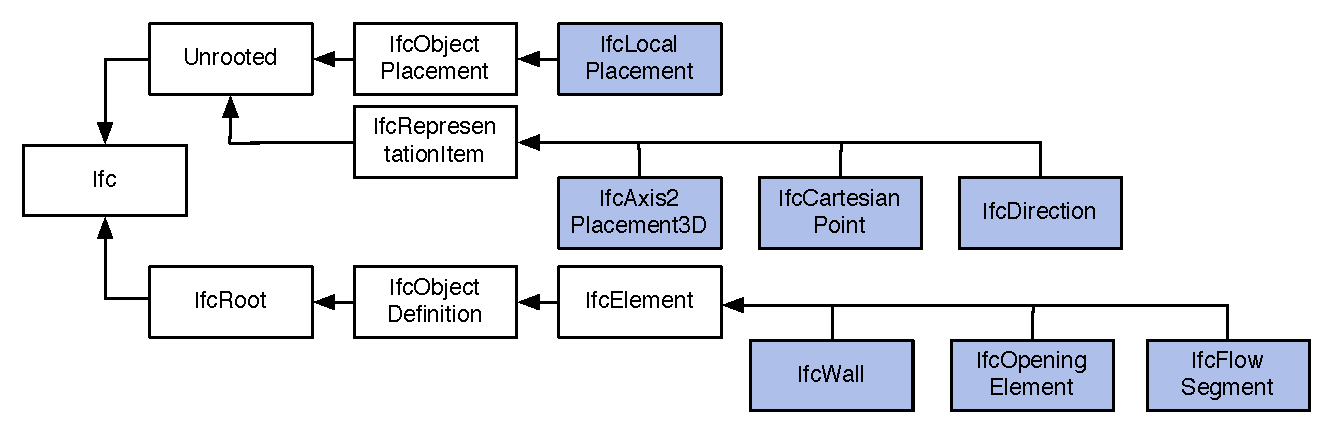
\includegraphics[width=120mm]{images/IfcHeirachy.pdf}
    \caption{A graphical representation of the subset used, excluding relational objects.}
    \label{fig:ifcheirachy}
\end{figure}

\subsection{Eclipse Modeling Framework and Ecore}
The Eclipse Modeling Framework (EMF project) is a modeling framework and code generation facility for building tools and other applications based on a structured data model\cite{emf}. EMF is capable of producing a Java object graph from a model instance described in XMI. For meta modeling this instance EMF includes Ecore. Ecore is a meta modeling tool, allowing the user to describe and build meta models for their domain. Furthermore EMF has several transformation tools, enabling transformation from either one Ecore model to another or from Ecore model directly to a textual format.

\subsection{Conclusion}
In this section the basic ideas behind digital representation of buildings was presented. We focus on BIM for this representation and the IFC format to represent BIM. To solve the problem explained in sections \ref{sec:workflow} and \ref{sec:solution_domain_definition}, a way to edit a subset of IFC. This will be done with model to model transformations using tools supplied by EMF.